\section{哈密顿回路与旅行商}
\label{sec:04-Discrete-Mathematics/03-Graph-Theory/08}

立项会上摆着两个需求。一个来自市政：辖区每条街道都要巡查一遍，别重复。另一个来自销售：名单上每个客户都要拜访一次，别重复。听起来是同一类活，报价和排期也就照着同一个模子填了。

第一个需求上一节已经解决：数一遍度数奇偶，线性时间给出答案，还顺带产出路线。第二个需求至今没有人知道怎么在多项式时间内回答。两句话只差一个词——边换成顶点——而它们之间隔着一整个复杂度阶级。这个对照值得比本节任何一个算法都记得牢。

\subsection{同一张图，两个答案}

经过每个顶点恰好一次并回到起点的环叫哈密顿回路，不要求闭合的叫哈密顿路径。名字来自 1857 年 Hamilton 推销的一种玩具：在正十二面体的二十个顶点上找一条沿棱经过每点一次的环游。玩具没卖动，问题留了下来。

用上一节末尾那张图就能把两个问题的差别看清楚。

\begin{center}
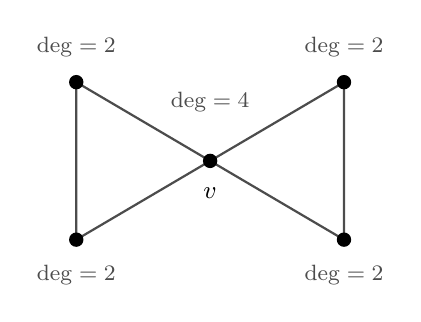
\begin{tikzpicture}[x=1cm,y=1cm,font=\small]
  \draw[thick,black!70] (0,0) -- (-1.7,1.0) -- (-1.7,-1.0) -- (0,0);
  \draw[thick,black!70] (0,0) -- (1.7,1.0) -- (1.7,-1.0) -- (0,0);
  \fill (0,0) circle (2.6pt); \node[below] at (0,-0.22) {\(v\)};
  \fill (-1.7,1.0) circle (2.6pt); \fill (-1.7,-1.0) circle (2.6pt);
  \fill (1.7,1.0) circle (2.6pt); \fill (1.7,-1.0) circle (2.6pt);
  \node[black!70,font=\footnotesize] at (-1.7,1.45) {\(\deg=2\)};
  \node[black!70,font=\footnotesize] at (1.7,1.45) {\(\deg=2\)};
  \node[black!70,font=\footnotesize] at (-1.7,-1.45) {\(\deg=2\)};
  \node[black!70,font=\footnotesize] at (1.7,-1.45) {\(\deg=2\)};
  \node[black!70,font=\footnotesize] at (0,0.75) {\(\deg=4\)};
\end{tikzpicture}

\emph{两个三角形共用顶点 \(v\)。度数全偶且连通，欧拉回路存在，六条边一笔画得完。但任何经过全部五个顶点的环都必须两次经过 \(v\)——左边三角形进出一次、右边三角形进出一次——所以哈密顿回路不存在。判定左边那件事只要数度数，判定右边那件事得动脑子。}
\end{center}

一般图上判定哈密顿回路是否存在，是 NP 完全问题；哈密顿路径同样。这个说法的实际含义有三层：至今没有人找到多项式时间的判定算法；它与可满足性、团、背包等一大批难题彼此等价，任何一个若被攻破其余全部跟着倒；半个多世纪的高强度研究之后，人们普遍相信这样的算法不存在。定义与归约的细节见\hyperref[sec:09-Convex-Optimization/09-Complexity-and-Approximation/01]{``P、NP 与 NP-hard：给问题按计算难度分类''}。

\subsection{证书的不对称}

要理解难在哪里，把``找答案''和``验答案''分开看。

有人递来一条候选环游 \(v_1,v_2,\ldots,v_n,v_1\)，检验它是不是哈密顿回路轻而易举：每个顶点恰好出现一次，每对相邻顶点之间确有边。这就是它属于 NP 的含义——肯定答案有短证书。难的是自己找到这条环。更难的是当答案为``不存在''时，拿出一份短的、可核对的否定证明。

欧拉问题在这一格上有东西：``顶点 \(u\) 的度数是奇数''就是一份一句话的否定证书，任何人一秒钟核完。哈密顿问题没有已知的对应物。这个空缺正是难度的来源，而不是难度的副产品。

{\def\LTcaptype{none}
\begin{longtable}{@{}lll@{}}
\toprule\noalign{}
 & 欧拉回路（走遍每条边） & 哈密顿回路（走遍每个顶点） \\
\midrule\noalign{}
\endhead
\bottomrule\noalign{}
\endlastfoot
充要判据 & 连通且度数全偶 & 至今没有 \\
判定代价 & \(O(\abs{V}+\abs{E})\) & NP 完全 \\
肯定证书 & 一条路线，线性时间核对 & 一条环游，多项式时间核对 \\
否定证书 & 一个奇度顶点 & 无通用形式 \\
构造 & 判据的证明即算法 & 与判定同样困难 \\
\end{longtable}
}

表里最值得盯着看的是最后两行右列。欧拉那一侧，判定与构造是同一件事；哈密顿这一侧，连``不存在''都说不清楚。两个问题的表述几乎对称，四项指标全不对称。

这件事对工程判断的价值超过任何一条具体算法。接到一个图上的需求，先别问用什么库，先问它是欧拉型还是哈密顿型——不可遗漏的对象是边还是顶点，是否要求经过一次而非至少一次。答案决定的不是实现难度，而是你该承诺``给出最优解''还是``给出一个说得清误差的近似解''。这个问题问在立项前，成本是十分钟；问在交付前，成本是整个项目。

\subsection{必要条件只能否定}

没有充要判据，一些必要条件仍然能快速排除掉一批图。

哈密顿图必连通，每个顶点度数至少为 2——回路要用两条不同的边进出每个顶点，所以出现孤立点或叶子就可以立刻收工。它也不能有割点：删掉 \(v\) 后若图碎成两块，哈密顿回路去掉 \(v\) 本该剩下一条经过其余全部顶点的路径，而一条路径跨不过互不相连的两块。上面那张双三角形图正是被这一条否掉的。更一般地，删去顶点集 \(S\) 后的连通分量数必须满足

\[
c(G-S)\le\abs{S}
\qquad\text{对每个非空 }S\subseteq V,
\]

因为从环上删掉 \(\abs{S}\) 个顶点至多把它切成 \(\abs{S}\) 段。二分图还多一项：回路在两侧交替行走，两侧顶点数必须相等。

这些检查全都是单向的。Petersen 图连通、三正则、没有割点，上述检查一条不落地通过，却没有哈密顿回路。``度数都不小、图看着挺结实''不构成存在性证明。同一种逻辑在下一节还会以另一副面孔出现：一族不变量可以否定，永远不能确认。

反过来也有单向的充分条件。Dirac 在 1952 年证明：\(n\ge 3\) 个顶点的简单图若每个顶点度数都不小于 \(n/2\)，则有哈密顿回路。Ore 在 1960 年把它放宽成：每对不相邻顶点的度数之和不小于 \(n\)。直觉是``密到绕不开''——取一条最长路径，端点的邻居必须全挤在这条路径上，否则接出去就更长；度数一大，挤到某处必然重叠，重叠处正好把路径首尾接成环。这类条件刻画的是稠密图。环 \(C_n\)（\(n\ge 5\)）自己就是哈密顿图，最小度却只有 2，远够不上门槛。Dirac 的阈值也一步都不能降：\(n\) 为偶数时取两个互不相连的 \(K_{n/2}\)，每点度数恰好是 \(n/2-1\)，图不连通，自然没有回路。

\subsection{指数时间也分层次}

``没有多项式算法''不等于只能盲目枚举 \(n!\) 种排列。旅行商问题的经典动态规划把状态取为 \(D(S,j)\)，含义是从固定起点出发、恰好访问过顶点集 \(S\)、当前停在 \(j\) 的最小代价。递推是

\[
D(S,j)=\min_{i\in S\setminus\set{j}}\bigl(D(S\setminus\set{j},i)+w_{ij}\bigr).
\]

这个 Held--Karp 算法需要约 \(O(n^{2}2^{n})\) 时间，仍是指数，却比 \(n!\) 好得多。指数因子的来源写在状态里：每个顶点只有``访问过''与``没访问过''两种身份，集合共 \(2^{n}\) 个。之所以只需记住集合而不必记住顺序，是因为两条访问过同一批顶点、停在同一处的前缀，对未来的选择完全等价，留代价小的那条就够了。动态规划扔掉的是与未来无关的历史。

分支定界、整数规划与割平面进一步用下界剪掉不可能更优的分支。最坏情形依旧困难，但结构化的实例常常远比最坏情形容易——复杂性结论说的是一类输入的最坏情形，不能替代对手上这批实例的分析。

\subsection{最优不可求时，一棵树给出两倍保证}

给每条边标上价格，就得到旅行商问题（TSP）：在带非负边权的完全图上求权最小的哈密顿回路。加权没有让问题变容易，判定版本``是否存在总价不超过 \(B\) 的环游''仍是 NP 完全的。

哈密顿回路怎样藏进 TSP，一句话就说完：原图里有的边赋权 1，没有的边补上并赋权 2。若最优环游总权不超过 \(n\)，它的每条边只能取权 1，那正是原图的哈密顿回路。所以一般 TSP 一旦能快速精确求解，哈密顿回路的判定也就跟着解决了。

实用的出路是求近似，而近似需要一个额外条件：三角不等式，即绕路不比直达便宜。几何距离满足它，用最短路距离补成的完全图也满足它。在这个前提下，\hyperref[sec:04-Discrete-Mathematics/03-Graph-Theory/03]{``树与生成树''}里的最小生成树就给出一个干净的 2-近似。

\begin{center}
\begin{tikzpicture}[x=1cm,y=1cm,font=\small]
  \draw[dashed,red!65!black,thick] (0,0) -- (2.2,0.4) -- (4.0,-0.6) -- (3.4,1.8) -- (1.4,2.0) -- (0,0);
  \draw[very thick,black!75] (0,0) -- (2.2,0.4);
  \draw[very thick,black!75] (2.2,0.4) -- (4.0,-0.6);
  \draw[very thick,black!75] (2.2,0.4) -- (3.4,1.8);
  \draw[very thick,black!75] (3.4,1.8) -- (1.4,2.0);
  \foreach \p in {(0,0),(2.2,0.4),(4.0,-0.6),(3.4,1.8),(1.4,2.0)}{\fill \p circle (2.6pt);}
  \node[black!75,font=\footnotesize] at (1.0,-0.55) {最小生成树};
  \node[red!65!black,font=\footnotesize] at (2.5,2.45) {抄近路后的环游};
\end{tikzpicture}

\emph{最优环游删掉任意一条边就是一棵生成树，所以最小生成树的权不超过 \(\mathrm{OPT}\)。把树的每条边走两遍得到一条覆盖全部顶点的闭合游走，权为树权的两倍；三角不等式允许跳过已访问过的顶点直接抄近路（虚线），近路只会更短。于是虚线这条哈密顿回路的权不超过 \(2\,\mathrm{OPT}\)。}
\end{center}

三条不等式串起来就是全部证明，值得逐条对账它们各自靠什么成立。第一条靠``删一边得生成树''，只用到最优环游是一个环。第二条只是把每条边数两遍，纯计数。第三条完全压在三角不等式上：若它失败，抄近路可能反而更贵——从 \(u\) 经 \(v\) 到 \(w\) 便宜，而 \(u\) 直达 \(w\) 极贵的情形并不违反任何图论公理。此时两倍保证不是稍微变差，而是整个失效。

度量情形下还能更好。Christofides 算法在最小生成树上找出奇度顶点，对它们做最小权完美匹配，把图补成全偶后取欧拉回路，再抄近路，保证不超过 \(3\,\mathrm{OPT}/2\)。这一串动作用上了本单元几乎所有零件：生成树给下界，匹配修奇偶，欧拉回路负责走遍边，最后才压成哈密顿回路。最近邻、2-opt 之类的启发式则是另一回事——在真实数据上常常很强，却没有统一的最坏情形比例，一条很短的实验路线证明不了接近最优。

想说清``离最优还有多远''，必须同时握住两侧：可行解给出上界 \(U\)，松弛或下界方法给出 \(L\)，于是 \(L\le\mathrm{OPT}\le U\)。最小生成树权就是一种下界，1-tree 与整数规划松弛更强。两端相等时最优性被证明，否则只能老实报告区间。用上界与下界把最优值夹住，是\hyperref[ch:075]{``对偶：为最优性建立下界证书''}反复使用的手法，这里只是它在组合问题上的一次早期露面。

\subsection{建模时别把两个问题混着说}

完全图上的``每城一次''允许实际道路经过别的城市，代价定义为最短路距离；若业务规定路过也算拜访，模型就得改。时间窗、车辆容量、多个仓库、非对称路价分别通向另外几个问题，本节的定理与近似比不能直接搬。还要分清``找一条可行环''与``找最短环''：把缺失的边补成极大权重虽然能把存在性塞进优化模型，但算法返回的路线若真用了这类边，那只是在告诉你原图没有可行环，不能当成一条真实路线报出去。

欧拉与哈密顿的对照最终指向一件事：难度藏在结构里，不在表述里，看上去平行的两句话可以落在计算世界的两个不同区域。下一节问的是同一类问题的另一个版本——一张图能不能画在纸上而边不交叉。这同样与你怎么画无关，而答案又一次由一个简单的计数式封死。
